\documentclass[border=4pt]{standalone}
\usepackage{fontspec}
\usepackage{amsmath}
\usepackage{unicode-math}
\setmainfont{Latin Modern Roman}
\setmathfont{Latin Modern Math}
\usepackage{pgfplots}
\usepackage{pgfplotstable}
\pgfplotsset{compat=1.18}
\usepackage{tkz-euclide}
\usetikzlibrary{arrows.meta,calc,angles,quotes,patterns,3d,backgrounds}
\definecolor{ink}{HTML}{123428}
\definecolor{asy}{HTML}{475569}
\definecolor{mint}{HTML}{86e0bd}
\tikzset{asym/.style={asy, line width=0.9pt, dash pattern=on 5pt off 3.5pt},
         guide/.style={gray!70, line width=0.6pt, densely dotted},
         dot/.style={circle, inner sep=0pt, minimum size=5pt, draw=white, line width=0.5pt},
         odot/.style={circle, inner sep=0pt, minimum size=5.5pt, fill=white, line width=1pt},
         lab/.style={font=\footnotesize, inner sep=1.5pt, text=ink}}
\begin{document}
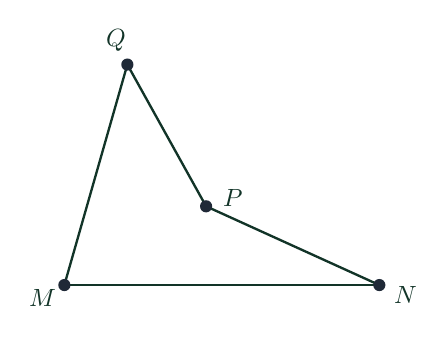
\begin{tikzpicture}
\draw[ink, line width=0.85pt] (0.000,0.000) -- (4.000,0.000);
\draw[ink, line width=0.85pt] (4.000,0.000) -- (1.800,1.000);
\draw[ink, line width=0.85pt] (1.800,1.000) -- (0.800,2.800);
\draw[ink, line width=0.85pt] (0.800,2.800) -- (0.000,0.000);
\fill[color={rgb,255:red,31;green,41;blue,55}] (0.000,0.000) circle (2.2pt);
\fill[color={rgb,255:red,31;green,41;blue,55}] (4.000,0.000) circle (2.2pt);
\fill[color={rgb,255:red,31;green,41;blue,55}] (1.800,1.000) circle (2.2pt);
\fill[color={rgb,255:red,31;green,41;blue,55}] (0.800,2.800) circle (2.2pt);
\node[font=\small, text=ink, inner sep=0.5pt] at (-0.295,-0.170) {$M$};
\node[font=\small, text=ink, inner sep=0.5pt] at (4.315,-0.127) {$N$};
\node[font=\small, text=ink, inner sep=0.5pt] at (2.123,1.108) {$P$};
\node[font=\small, text=ink, inner sep=0.5pt] at (0.658,3.109) {$Q$};
\end{tikzpicture}
\end{document}
